Model categories are categories with weak equivalences,
together with some extra data, namely
a class $\cat{Cof}$ of \emph{cofibrations},
and a class $\cat{Fib}$ of \emph{fibrations}.
This extra data will help us in computations related to $∞$-categories. 
Recall that we have a mind-map
\[ \begin{tikzcd}[column sep=3em,row sep=2em]
    \overset{\text{model category}}{(\cat C,\cat W,\cat{Cof},\cat{Fib})} \ar[dr,"\text{present }(\text{easier})"] \\
    (\cat C,\cat W) \ar[u,dashed,"\text{find a structure}"] \ar[r,"\text{localise}","(\text{hard to describe})"']
    & \infty\text{-category }\cat C[\cat W^{-1}] \ar[d,"\text{forget}"] \\
    & \text{ordinary category }\cat C[\cat W^{-1}]
\end{tikzcd} \]

Model categories have two main advantages in such computations:
\begin{itms}
    \item \textbf{Homotopies between morphisms} are easily described.
    Normally we only know which morphisms are weak equivalences;
    we do not know which morphisms become homotopic after localisation.
    However, in model categories, we can see such homotopies,
    and we can even see all the higher dimensional homotopies,
    just like we are working with topological spaces.
    As a result, the localisation $\cat C[\cat W^{-1}]$
    will have a good description as the \emph{homotopy category} of $\cat C$.

    \item \textbf{Derived functors} are very easy to compute.
    They will be defined later in this section.
    For example, homotopy limits and colimits are examples of derived functors.
\end{itms}

\subsection{Definition and examples}

Recall from algebraic topology
that a map $p\:X\to Y$ of topological spaces is called a \term{Hurewicz fibration}
if for any space $A$ and any diagram (without the dashed arrow)
\[ \begin{tikzcd}
    A\times\{0\}\ar[r]\ar[d] & X\ar[d,"p"] \\
    A\times I\ar[r]\ar[ur,dashed] & Y\rlap{\ ,}
\end{tikzcd} \]
there exists a dashed arrow making the diagram commute.
A map $i\:A\to B$ is called a \term{Hurewicz cofibration}
if for any space $Y$ and any diagram
\[ \begin{tikzcd}
    A\ar[r]\ar[d,"i"'] & Y^I\ar[d] \\
    B\ar[r]\ar[ur,dashed] & Y^{\{0\}}\rlap{\ ,}
\end{tikzcd} \]
there exists a dashed arrow making the diagram commute,
where $Y^I$ denotes the space of all maps $I\to Y$
equipped with the compact open topology.

\begin{definition}
    Let $\cat C$ be a category, and let $J\subset\operatorname{Mor}(\cat C)$ be a class of morphisms.
    We say that a map $p\:X\to Y$ in $\cat C$ has the \term{right lifting property} against $J$,
    if for any diagram
    \[ \begin{tikzcd}
        A\ar[r]\ar[d] & X\ar[d,"p"] \\
        B\ar[r]\ar[ur,dashed] & Y
    \end{tikzcd} \]
    in $\cat C$, where the map $A\to B$ is in $J$,
    there exists a dashed arrow making the diagram commute.
    The class of all arrows $p$ with this property is denoted by $\operatorname{RLP}(J)$.

    Dually, a map $i\:A\to B$ in $\cat C$ has the \term{left lifting property} against $J$,
    if for any diagram
    \[ \begin{tikzcd}
        A\ar[r]\ar[d,"i"'] & X\ar[d] \\
        B\ar[r]\ar[ur,dashed] & Y
    \end{tikzcd} \]
    in $\cat C$, where the map $X\to Y$ is in $J$,
    there exists a dashed arrow making the diagram commute.
    The class of all arrows $i$ with this property is denoted by $\operatorname{LLP}(J)$.
\end{definition}

For example, we have by definition
\[ \begin{aligned}
    \{\text{Hurewicz fibrations}\}
    &=\operatorname{RLP}\{A\times\{0\}\hookrightarrow A\times I\},\\
    \{\text{Hurewicz cofibrations}\}
    &=\operatorname{LLP}\{Y^I\twoheadrightarrow Y^{\{0\}}\}.
\end{aligned}\]

As an exercise, the reader can show that
$\operatorname{RLP}(\operatorname{LLP}(\operatorname{RLP}(J)))=\operatorname{RLP}(J)$,
so that if we put $\cat R\coloneq\operatorname{RLP}(J)$ and
$\cat L\coloneq\operatorname{LLP}(\operatorname{RLP}(J))$,
then $\cat L=\operatorname{LLP}(\cat R)$ and $\cat R=\operatorname{RLP}(\cat{L})$.

\begin{definition}
    A \term{weak factorisation system} is a triple $(\cat C,\cat L,\cat R)$,
    where $\cat C$ is a category, and
    $\cat L,\cat R\subset\operatorname{Mor}(\cat C)$ are two classes of morphisms,
    such that
    \begin{itms}
        \item $\cat L=\operatorname{LLP}(\cat R)$ and $\cat R=\operatorname{RLP}(\cat{L})$.
        \item Every morphism $f\:A\to B$ in $\cat C$ can be factored into
        \[A\xrightarrow lX\xrightarrow rB,\]
        where $l\in\cat L$ and $r\in\cat R$.
        Moreover, we require that the factorisation is functorial in $f$.
    \end{itms}
\end{definition}

For example, let $\cat{HCof}$, $\cat{HFib}$ and $\cat{HoEq}$
denote the class of closed Hurewicz cofibrations,
the class of Hurewicz fibrations, and the class of homotopy equivalences, respectively.
We will see that the triples
$(\cat{Top},\cat{HCof}\cap\cat{HoEq},\cat{HFib})$
and
$(\cat{Top},\cat{HCof},\cat{HFib}\cap\cat{HoEq})$
both form weak factorisation systems.

\begin{proposition}
    Let $(\cat{C},\cat{L},\cat{R})$ be a weak factorisation system.
    \begin{itms}
        \item $\cat{L}$ and $\cat{R}$ contain all isomorphisms in $\cat{C}$.
        \item $\cat{L}$ and $\cat{R}$ are closed under composition.
        \item $\cat{L}$ is preserved by pushouts and $\cat{R}$ is preserved by pullbacks.
    \end{itms}
\end{proposition}

\begin{proof}
    Exercise for the reader.
\end{proof}

\begin{definition}
    A \term{model category} $(\cat{C},\cat{W},\cat{Cof},\cat{Fib})$
    is a category $\cat{C}$ with
    three distinguished classes of morphisms
    $\cat{W},\cat{Cof},\cat{Fib}\subset\operatorname{Mor}(\cat{C})$,
    such that
    \begin{itms}
        \item $\cat{C}$ admits all small colimits and limits.
        \item $(\cat{C},\cat{W})$ is a category with weak equivalences.
        \item $(\cat{C},\cat{Cof}\cap\cat{W},\cat{Fib})$ is a weak factorisation system.
        \item $(\cat{C},\cat{Cof},\cat{Fib}\cap\cat{W})$ is a weak factorisation system.
    \end{itms}
\end{definition}

We shall now introduce some terminology.
\begin{itms}
    \item Morphisms in $\cat W$ are called \emph{weak equivalences}.
    \item Morphisms in $\cat{Cof}$ are called \emph{cofibrations}.
    \item Morphisms in $\cat{Fib}$ are called \emph{fibrations}.
    \item Morphisms in $\cat{Cof}\cap\cat W$ are called \emph{trivial cofibrations},
    or \emph{acyclic cofibrations}.
    \item Morphisms in $\cat{Fib}\cap\cat W$ are called \emph{trivial fibrations},
    or \emph{acyclic fibrations}.
    \item An object $X\in\cat C$ is \emph{cofibrant} if the map $\emptyset\to X$ is a cofibration,
    where $\emptyset$ denotes the initial object of $\cat C$.
    The initial object exists because it is the empty colimit.
    \item An object $X\in\cat C$ is \emph{fibrant} if the map $X\to*$ is a fibration,
    where $*$ denotes the terminal object of $\cat C$.
    The terminal object exists because it is the empty limit.
\end{itms}

Note that $\cat{Cof}$ and $\cat{Fib}$ determine each other,
since in a weak factorisation system,
the two classes of morphisms determine each other.
Note also that cofibrations and trivial cofibrations
are preserved by pushouts,
and fibrations and trivial fibrations
are preserved by pullbacks.

Let us look at some examples.
It is often very tedious to verify the axioms of a model category,
so we will present the results without giving proofs.

\begin{example}
    The \term{Hurewicz model structure} on $\cat{Top}$ is defined as follows.
    \begin{itms}
        \item $\cat{W}$ is the class of homotopy equivalences.
        \item $\cat{Cof}$ is the class of closed Hurewicz cofibrations.
        \item $\cat{Fib}$ is the class of Hurewicz fibrations. \varqed
    \end{itms}
\end{example}

\begin{example}
    The \term{Quillen model structure} on $\cat{Top}$ is defined as follows.
    \begin{itms}
        \item $\cat{W}$ is the class of weak homotopy equivalences.
        \item $\cat{Fib}:=\operatorname{RLP}\{D^n\times\{0\}\hookrightarrow D^n\times I\mid n\geq0\}$
        is the class of Serre fibrations.
        \item $\cat{Fib}\cap\cat W=\operatorname{RLP}\{S^{n-1}\hookrightarrow D^n\mid n\geq0\}$.
        This is an alternative characterisation of $\cat{Fib}\cap\cat W$.
        \item $\cat{Cof}$ is determined by $\cat{Cof}=\operatorname{LLP}(\cat{Fib}\cap\cat W)$.
        In particular, the maps $S^{n-1}\hookrightarrow D^n$ are cofibrations.
    \end{itms}
    In this model category, every topological space is fibrant.
    All CW complexes are cofibrant,
    because cofibrations are preserved by pushouts,
    and preserved by composition and sequential colimits. \varqed
\end{example}

In the sequel, we will always use the Quillen model structure,
instead of the Hurewicz model structure.

\begin{example}
    The \term{projective model structure} on $\cat{Ch}_R$ is defined as follows.
    \begin{itms}
        \item $\cat{W}$ is the class of quasi-isomorphisms.
        \item $\cat{Fib}$ is the class of degreewise surjections.
    \end{itms}
    In this model category, every cochain complex is fibrant.
    Any bounded-above cochain complex consisting of projective modules,
    e.g.\ a projective resolution of an $R$-module,
    is cofibrant. \varqed
\end{example}

\begin{example}
    The \term{injective model structure} on $\cat{Ch}_R$ is defined as follows.
    \begin{itms}
        \item $\cat{W}$ is the class of quasi-isomorphisms.
        \item $\cat{Cof}$ is the class of degreewise injections.
    \end{itms}
    In this model category, every cochain complex is cofibrant.
    Any bounded-below cochain complex consisting of injective modules,
    e.g.\ an injective resolution of an $R$-module,
    is fibrant. \varqed
\end{example}

As can be seen in these examples, 
\term{cofibrant-fibrant objects}, i.e.\ objects that are both cofibrant and fibrant,
are special objects that
behave like CW complexes or projective/injective resolutions.
We will soon see that these objects
have much better properties than others.
However, it turns out that every object
is weakly equivalent to a cofibrant-fibrant object.

\begin{construction}
    Let $\cat C$ be a model category.
    By the axioms for a model category,
    for any $X\in\cat C$, we may factorise the map $\emptyset\to X$ into
    \[ \emptyset\xrightarrow{\in\cat{Cof}}QX\xrightarrow{\in\cat{Fib}\cap\cat{W}}X. \]
    Then $QX$ is a cofibrant object that is weakly equivalent to $X$.
    Moreover, $Q$ is a functor, and is called the \term{cofibrant replacement} functor.

    Dually, we may factorise the map $X\to *$ into
    \[ X\xrightarrow{\in\cat{Cof}\cap\cat{W}}RX\xrightarrow{\in\cat{Fib}}*. \]
    Then $RX$ is a fibrant object that is weakly equivalent to $X$.
    Moreover, $R$ is a functor, and is called the \term{fibrant replacement} functor.

    More generally, any functor $Q\:\cat{C}\to\cat{C}$
    (resp.\ $R\:\cat{C}\to\cat{C}$) with the properties described above
    will be called a \term{cofibrant replacement} (resp.\ \term{fibrant replacement}) functor.

    As an exercise,
    the reader can show that the objects $RQX$ and $QRX$ are both cofibrant-fibrant. \varqed
\end{construction}

\subsection{Homotopy category}

In this section, we aim to recover ``homotopies'' from the axioms of a model category.
In topology, a homotopy between maps $X\to Y$ is given by a map
\[ X\times I\to Y,\quad\text{or}\quad X\to Y^I. \]
In a model category, we define homotopies
by considering objects that behave like $X\times I$ or $Y^I$.

\begin{definition}
    Let $\cat C$ be a model category,
    and let $X\in\cat{C}$ be an object.
    \begin{itms}
        \item A \term{cylinder object} $\operatorname{Cyl}(X)$ for $X$ is a factorisation
        of the codiagonal map $\nabla_X:=(\mathbb1,\mathbb1)\:X\sqcup X\to X$ as
        \[ \begin{tikzcd}
            X\sqcup X\ar[rr,"\nabla_X"]\ar[dr,"\cat{Cof}\ni i"'] &   & X \\
            & \operatorname{Cyl}(X)\rlap{\ .}\ar[ur,"p\in\cat{W}"'] &   
        \end{tikzcd} \]
        The cylinder object is said to be \term{very good} if moreover $p\in\cat{Fib}\cap\cat{W}$.

        \item A \term{path space object} $\operatorname{Path}(X)$ for $X$ is a factorisation
        of the diagonal map $\Delta_X:=(\mathbb1,\mathbb1)\:X\to X\times X$ as
        \[ \begin{tikzcd}
            X\ar[rr,"\Delta_X"]\ar[dr,"\cat{W}\ni i"'] &   & X\times X \\
            & \operatorname{Path}(X)\rlap{\ .}\ar[ur,"p\in\cat{Fib}"'] &   
        \end{tikzcd} \]
        The path space object is said to be \term{very good} if moreover $i\in\cat{Cof}\cap\cat{W}$.
    \end{itms}
\end{definition}

These are objects that behave like $X\times I$ and $X^I$
in topology, respectively.
By the axioms of a model category, we can always find
very good cylinder and path space objects
for any object $X$.

\begin{definition}
    Let $f,g\:X\to Y$ be two morphisms in $\cat C$.
    \begin{itms}
        \item A \term{left homotopy} from $f$ to $g$ is a morphism $\operatorname{Cyl}(X)\to Y$,
        such that the diagram
        \[ \begin{tikzcd}
            X\ar[r,"i_0"]\ar[dr,"f"'] & \operatorname{Cyl}(X)\ar[d] & X\ar[l,"i_1"']\ar[dl,"g"] \\
            & Y &   
        \end{tikzcd} \]
        commutes. In this case, we say that
        $f$ and $g$ are \term{left homotopic}.

        \item A \term{right homotopy} from $f$ to $g$ is a morphism $X\to\operatorname{Path}(Y)$,
        such that the diagram
        \[ \begin{tikzcd}
            & X\ar[dl,"f"']\ar[d]\ar[dr,"g"] &   \\
            Y & \operatorname{Path}(Y)\ar[l,"p_0"]\ar[r,"p_1"'] & Y
        \end{tikzcd} \]
        commutes. In this case, we say that
        $f$ and $g$ are \term{right homotopic}.
    \end{itms}
\end{definition}

In topology, left homotopies are equivalent to right homotopies.
We will soon show that this is also true
for cofibrant-fibrant objects,
but before that,
let us get familiar with the axiomatic way of doing homotopy theory
through an example.

\begin{example}
    If $f_0,f_1\:X\to Y$ are left homotopic maps,
    and $g_0,g_1\:Y\to Z$ are left homotopic maps,
    then $g_0\circ f_0$ and $g_1\circ f_1$ are left homotopic,
    provided that the canonical very good cylinder objects,
    i.e.\ those obtained from the functorial factorisation
    of the codiagonal maps of $X$ and $Y$,
    are used.
\end{example}

\begin{proof}
    In topology, we prove this obvious fact by considering the composition
    \[ X\times I\to X\times I\times I\to Y\times I\to Z, \]
    where the first map is induced from the diagonal map $I\hookrightarrow I\times I$,
    which is a path connecting the vertices $(0,0)$ and $(1,1)$.

    In the model category setting,
    we wish to get a series of maps
    \[ \operatorname{Cyl}(X)\to\operatorname{Cyl}(\operatorname{Cyl}(X))\to \operatorname{Cyl}(Y)\to Z, \]
    which gives the desired homotopy.
    Since we are using the canonical cylinder objects,
    we can regard $\operatorname{Cyl}$ as a functor.
    This gives the map $\operatorname{Cyl}(\operatorname{Cyl}(X))\to \operatorname{Cyl}(Y)$.
    Thus, the only problem now is to construct the first map
    $\operatorname{Cyl}(X)\to\operatorname{Cyl}(\operatorname{Cyl}(X))$,
    as ``a path connecting the vertices $(0,0)$ and $(1,1)$''.
    We do this by lifting in the diagram
    \[ \begin{tikzcd}
        X\sqcup X\ar[d,"\cat{Cof}\ni i"']\ar[r,"(i_0i_0\comma i_1i_1)"] & 
        \operatorname{Cyl}(\operatorname{Cyl}(X))\ar[d,"\in\cat{Fib}\cap\cat{W}"] \\
        \operatorname{Cyl}(X)\ar[r]\ar[ru,dashed] & X\rlap{\ .}
    \end{tikzcd} \]
    The reader can now readily check that
    the composition map $\operatorname{Cyl}(X)\to Z$
    does give a left homotopy between $g_0\circ f_0$ and $g_1\circ f_1$.
\end{proof}

\begin{proposition}
    Let $f,g\:X\to Y$ be two maps.
    If $X$ is cofibrant and $Y$ is fibrant, then
    $f$ and $g$ are left homotopic if and only if they are right homotopic.
    In this case, a homotopy exists
    for any cylinder object of $X$ and
    for any path space object of $Y$.
\end{proposition}

\begin{proof}
    Suppose that $h\:\operatorname{Cyl}(X)\to Y$ be a left homotopy from $f$ to $g$.
    The idea is to construct a map $k$ ``from $X\times I$ to $Y^I$'',
    as depicted in the diagram below.
    \[ 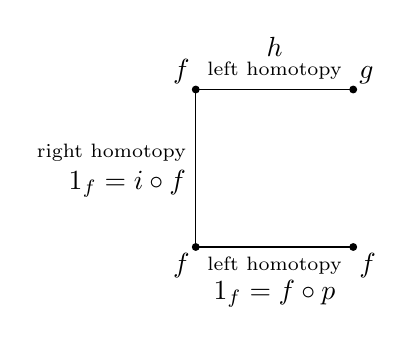
\begin{tikzpicture}[baseline=(base.base)]
        \draw (2,2)--(0,2)--(0,0)--(2,0);
        \fill (0,0) circle (.05);
        \fill (0,2) circle (.05);
        \fill (2,0) circle (.05);
        \fill (2,2) circle (.05);
        
        \node[anchor=south east,inner sep=2pt] at (0,2) {$f$};
        \node[anchor=north east,inner sep=2pt] at (0,0) {$f$};
        \node[anchor=north west,inner sep=2pt] at (2,0) {$f$};
        \node[anchor=south west,inner sep=2pt] at (2,2) {$g$};
        \node[anchor=south] at (1,2) {\scriptsize left homotopy};
        \node[anchor=south] at (1,2.3) {$h$};
        \node[anchor=east] at (0,1.2) {\scriptsize right homotopy};
        \node[anchor=east] at (0,.8) {$\mathbb{1}_f=i \circ f$};
        \node[anchor=north] at (1,0) {\scriptsize left homotopy};
        \node[anchor=north] at (1,-.3) {$\mathbb{1}_f=f \circ p$};
        \node(base) at (0,1) {\phantom{0}};
    \end{tikzpicture} 
    \quad \overset{\text{fill}}{\Longrightarrow} \quad
    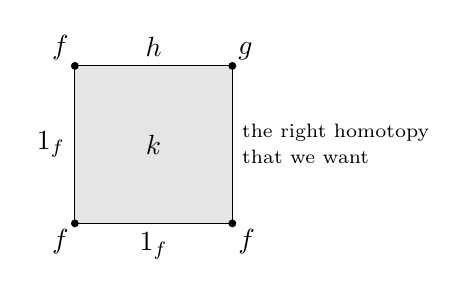
\begin{tikzpicture}[baseline=(base.base)]
        \fill[black!10] (0,0) rectangle (2,2);
        \draw (2,2)--(0,2)--(0,0)--(2,0)--cycle;
        \fill (0,0) circle (.05);
        \fill (0,2) circle (.05);
        \fill (2,0) circle (.05);
        \fill (2,2) circle (.05);
        
        \node[anchor=south east,inner sep=2pt] at (0,2) {$f$};
        \node[anchor=north east,inner sep=2pt] at (0,0) {$f$};
        \node[anchor=north west,inner sep=2pt] at (2,0) {$f$};
        \node[anchor=south west,inner sep=2pt] at (2,2) {$g$};
        \node[anchor=south] at (1,2) {$h$};
        \node[anchor=east] at (0,1) {$\mathbb{1}_f$};
        \node[anchor=north] at (1,0) {$\mathbb{1}_f$};
        \node[anchor=west] at (2,1.15) {\scriptsize the right homotopy};
        \node[anchor=west] at (2,.85) {\scriptsize that we want};
        \node at (1,1) {$k$};
        \node(base) at (0,1) {\phantom{0}};
    \end{tikzpicture} \]
    This idea is realised by lifting in the diagram
    \[ \begin{tikzcd}
        X \ar[d,"\cat{Cof}\cap\cat{W} \ni i_0"'] \ar[r,"i\circ f"] &
        \operatorname{Path}(Y) \ar[d,"\in\cat{Fib}"] \\
        \operatorname{Cyl}(X) \ar[r,"(f\circ p\comma h)"'] \ar[ur,dashed,"k"] &
        Y \times Y \rlap{\ .}
    \end{tikzcd} \]
    The reader should check the details implicit in the diagram,
    making use of the assumption that $X$ is cofibrant.
    The composition
    \[ X \xrightarrow{i_1} \operatorname{Cyl}(X) \xrightarrow{k} \operatorname{Path}(Y) \]
    then gives the desired right homotopy.

    Moreover, note that the path object $\operatorname{Path}(Y)$ above 
    was chosen arbitrarily. Therefore, being left homotopic implies 
    being right homotopic with respect to any path object.
    
    Dually, one shows that being right homotopic implies 
    being left homotopic with respect to any cylinder object.
\end{proof}

This proposition shows that
homotopy is a really nice property to work with,
at least for the cofibrant-fibrant objects.
As an exercise, the reader can show that
under the above conditions,
being homotopic is an equivalence relation for maps $X\to Y$.
Thus, we can take homotopy classes of maps and
define the homotopy category.

\begin{definition}
    The \term{homotopy category} of $\cat{C}$ is a category $\Ho(\cat{C})$, with
    \begin{itms}
        \item Objects: the cofibrant-fibrant objects of $\cat{C}$.
        \item Morphisms: homotopy classes of morphisms in $\cat{C}$.
    \end{itms}
\end{definition}

Do not forget that we study model categories
in order to study localisations.
And here is the key result:

\begin{theorem}\label{thm-2-a}
    We have an equivalence of categories
    \[\Ho(\cat{C})\simeq\cat{C}[\cat W^{-1}].\]
\end{theorem}

The proof of this theorem depends on the following fact.

\begin{proposition}[Whitehead's Theorem]\label{thm-2-w}
    Suppose $X,Y\in\cat C$ are cofibrant-fibrant objects.
    Then a morphism $f\:X\to Y$ is a weak equivalence
    if and only if it is a homotopy equivalence,
    i.e.\ it has a homotopy inverse.
\end{proposition}

\begin{proof}
    1. If $f \in \cat{Fib}\cap\cat{W}$,
    then $f$ has a right inverse, as we can lift in the diagram 
    \[ \begin{tikzcd}
        \emptyset \ar[r] \ar[d,"\cat{Cof}\ni"'] &
        X \ar[d,"f\in\cat{Fib}\cap\cat{W}"] \\
        Y \ar[ur,dashed,"g"] \ar[r,equals] & Y \rlap{\ .}
    \end{tikzcd} \]
    We have to show that $g$ is a homotopy inverse of $f$,
    and it suffices to show that $g\circ f$ is homotopic to $\mathbb{1}_X$.
    This is done by lifting in the diagram 
    \[ \begin{tikzcd}
        X\sqcup X \ar[r,"(g\circ f\comma\mathbb{1})"] \ar[d,"\cat{Cof}\ni"'] &
        X \ar[d,"f\in\cat{Fib}\cap\cat{W}"] \\
        \operatorname{Cyl}(X) \ar[ur,dashed] \ar[r,"f\circ p"] & Y\rlap{\ .}
    \end{tikzcd} \]

    2. If $f \in \cat{Cof}\cap\cat{W}$,
    then a dual argument will do.

    3. For a general $f\in\cat{W}$,
    we may factorise it into a cofibration and a trivial fibration.
    The cofibration is automatically trivial by two-out-of-three.
\end{proof}

\begin{proof}[Proof of \textup{(\ref{thm-2-a})}]
    By (\ref{thm-2-w}), the functor 
    \[ \cat{C} \xrightarrow{RQ} \cat{C}_{\mathrm{cf}} \to \Ho(\cat{C}) \]
    sends $\cat{W}$ to isomorphisms, inducing a functor
    from $\cat{C}[\cat W^{-1}]$ to $\Ho(\cat{C})$,
    which is clearly full and essentially surjective.
    We leave it to the reader to show that it is faithful
    (in the same way as we proved (\ref{thm-1-htop})).
\end{proof}

\begin{remark}
    We have noted that $\Ho(\cat C)$
    is the first layer of information obtained from localisation.
    The full information is retained in an $(\infty,1)$-category.
    We will see that model categories are capable of providing
    such higher structures,
    through a construction called a \term{framing}.
    This construction is analogous to $X\times\Delta^n$ and $X^{\Delta^n}$,
    in order to describe higher homotopies in a model category.
    See \cite[Chapter~5]{hovey} for details. \varqed
\end{remark}

\subsection{Derived functors}

Recall that in homological algebra,
derived functors are a way of passing a functor
between abelian categories $F\:\cat{A}\to\cat{B}$
to a functor between derived categories $\cat{D}(\cat{A})\to\cat{D}(\cat{B})$.
This is a special case of the following construction.

For a model category $\cat C$,
denote the subcategory of $\cat C$
consisting of cofibrant (resp.\ fibrant, cofibrant-fibrant) objects
by $\cat C_{\mathrm c}$ (resp.\ $\cat C_{\mathrm f}$, $\cat C_{\mathrm{cf}}$).

\begin{definition}
    Let $F\:\cat C\to\cat D$ be a functor,
    where $\cat C$ is a model category and 
    $\cat D$ is a category with weak equivalences.
    \begin{itms}
        \item If $F$ preserves weak equivalences, then $F$ induces a functor
        \[ \Ho(F)\:\Ho(\cat C)\to\Ho(\cat D). \]
        This is called the \term{total derived functor} of $F$.
        \item If $F|_{\cat C_{\mathrm c}}$ preserves weak equivalences,
        then there is a diagram
        \[\begin{tikzcd}
            \cat C\ar[d]\ar[r,"Q"] & \cat C_{\mathrm c}\ar[d]\ar[r,"F"] & \cat D\ar[d] \\
            \Ho(\cat C)\ar[r,equals] & \Ho(\cat C)\ar[r,"\mathbb LF"]
            & \Ho(\cat D)\rlap{\ ,}
        \end{tikzcd}\]
        which commutes up to natural isomorphisms,
        where $Q$ is any cofibrant replacement functor of $\cat C$.
        The functor $\mathbb LF$ is called the \term{left derived functor} of $F$.
        For any $X\in\cat C$, we have the formula
        \[ \mathbb LF(X)\simeq F(QX) \]
        in $\Ho(\cat D)$.
        \item If $F|_{\cat C_{\mathrm f}}$ preserves weak equivalences,
        then there is a diagram
        \[\begin{tikzcd}
            \cat C\ar[d]\ar[r,"R"] & \cat C_{\mathrm f}\ar[d]\ar[r,"F"] & \cat D\ar[d] \\
            \Ho(\cat C)\ar[r,equals] & \Ho(\cat C)\ar[r,"\mathbb RF"]
            & \Ho(\cat D)\rlap{\ ,}
        \end{tikzcd}\]
        which commutes up to natural isomorphisms,
        where $R$ is any fibrant replacement functor of $\cat C$.
        The functor $\mathbb RF$ is called the \term{right derived functor} of $F$.
        For any $X\in\cat C$, we have the formula
        \[ \mathbb RF(X)\simeq F(RX) \]
        in $\Ho(\cat D)$.
    \end{itms}
\end{definition}

\begin{example}
    In the category of cochain complexes with the injective model structure,
    the cofibrant replacement functor is taking projective resolutions.
    Thus the left derived functors defined above coincides with
    the standard definition in homological algebra.

    Similarly, in the category of cochain complexes with the projective model structure,
    the fibrant replacement functor is taking injective resolutions,
    which defines right derived functors. \varqed
\end{example}

\subsection{Derived adjunctions}

As we have seen, not all functors have derived functors.
In this subsection,
we give a criterion for an adjoint pair to both have derived functions,
so that their derived functors also form an adjoint pair.

\begin{definition}
    Let $\cat C,\cat D$ be two model categories,
    and let $(F\dashv G)$ be a pair of adjoint functors between them.
    Then $(F\dashv G)$ is called a \term{Quillen adjunction}
    if $F$ preserves cofibrations and trivial cofibrations.
\end{definition}

Note that $F$ preserves cofibrations iff $G$ preserves trivial fibrations,
and $F$ preserves trivial cofibrations iff $G$ preserves fibrations.

\begin{lemma}[Ken Brown]
    Let $F\:\cat C\to\cat D$ be a functor between two model categories.
    If $F|_{\cat C_{\mathrm c}}$ preserves trivial cofibrations,
    then $F|_{\cat C_{\mathrm c}}$ preserves weak equivalences.
\end{lemma}

\begin{proof}
    Omitted. See \cite[Lemma~1.1.12]{hovey}.
\end{proof}

\begin{corollary}
    If $(F\dashv G)$ is a Quillen adjunction
    between two model categories $\cat C$ and $\cat D$,
    then $\mathbb LF$ and $\mathbb RG$ exist.
    Moreover, $(\mathbb LF\dashv\mathbb RG)$
    is an adjunction between the homotopy categories $\Ho(\cat C)$ and $\Ho(\cat D)$.
\end{corollary}

\begin{proof}
    By Ken Brown's lemma, the derived functors $\mathbb LF$ and $\mathbb RG$ exist.
    To show that they form an adjunction, we have to show that the isomorphism 
    \[ \Hom_{\cat{C}}(FX,Y) \simeq \Hom_{\cat{D}}(X,GY) \]
    preserves homotopy classes for any $X\in\cat{D}_{\mathrm{cf}}$ and $Y\in\cat{C}_{\mathrm{cf}}$.
    This requires a little more work and we shall omit the details.
    See \cite[Lemma~1.3.10]{hovey}.
\end{proof}

\begin{definition}
    A Quillen adjunction $(F\dashv G)$
    is called a \term{Quillen equivalence} if
    $\mathbb LF$ and $\mathbb RG$ are equivalences of categories.
\end{definition}

A Quillen equivalence is not an equivalence of categories.
However, we will see that it induces an equivalence of 
$\infty$-categories obtained by localisation.
This will be a powerful tool to construct equivalences
between $\infty$-categories.

\begin{proposition}\label{thm-2-z}
    Let $(F\dashv G)$ be a Quillen equivalence
    between two model categories $\cat C$ and $\cat D$.
    Let $X\in\cat C$ be a cofibrant object,
    and let $Y\in\cat D$ be a fibrant object.
    Then the counit and unit maps 
    \[ X\to G R F X\quad\text{and}\quad F Q G Y\to Y \]
    are weak equivalences.
\end{proposition}

\begin{proof}
    Follows directly from the definitions.
\end{proof}
